\begin{table*}[t]
\centering
\resizebox{0.94\textwidth}{!}{
\begin{tabular}{lcccccccc}
\toprule
    \textbf{Model} & \textbf{GSM8K} & \textbf{MATH-500} & \textbf{AIME2024} & \textbf{AIME2025} & \textbf{AMC2023} & \textbf{OlympiadBench} & \textbf{AVG} \\
    \midrule
    LLaMA-3.1-8B-Base~\citep{dubey2024llama} & 7.58 & 3.20 & 0.00 & 0.00 & 4.22 & 1.19 & 2.70 \\
    \rowcolor{new_green!15}
    \texttt{\ \ + 20K Qwen-Distill-Data} & 62.47 & 29.40 & 0.00 & 0.00 & 12.81 & 6.81 & 18.58 \\
    \rowcolor{new_blue!15}
    \texttt{\ \ + 20K OSS-Distill-Data} & 75.89 & 54.20 & 4.38 & 6.46 & 37.34 & 23.85 & 33.69 \\
    \rowcolor{new_blue!15}
    \texttt{\ \ + 20K QwQ-Distill-Data} & 64.53 & 32.20 & 2.92 & 0.42 & 16.72 & 8.89 & 20.95 \\
    \rowcolor{new_purple!15}
    \texttt{\ \ + 20K OSS-\method{}} & 67.85  & 35.20  & 1.83  & 0.83  & 20.53  & 11.11  & 22.89 \\
    \rowcolor{new_purple!15}
    \texttt{\ \ + 20K QwQ-\method{}} & 66.41  & 35.00  & 2.08  & 0.63  & 20.16  & 10.37  & 22.44 \\
    \midrule
    Llama-3.1-8B-Instruct~\citep{dubey2024llama} & 75.89 & 35.20 & 4.17 & 1.04 & 23.59 & 12.00 & 25.32 \\
    \rowcolor{new_green!15}
    \texttt{\ \ + 20K Qwen-Distill-Data} & 76.50 & 39.80 & 4.38 & 1.04 & 25.63 & 19.70 & 27.84 \\
    \rowcolor{new_blue!15}
    \texttt{\ \ + 20K OSS-Distill-Data} & 79.00 & 60.80 & 10.83 & 7.71 & 47.03 & 30.22 & 39.27 \\
    \rowcolor{new_blue!15}
    \texttt{\ \ + 20K QwQ-Distill-Data} & 82.41 & 60.80 & 4.38 & 8.33 & 32.97 & 25.48 & 35.73 \\
    \rowcolor{new_purple!15}
    \texttt{\ \ + 20K OSS-\method{}} & 83.24 & 51.80 & 4.79 & 1.04 & 32.50 & 21.04 & 32.40  \\
    \rowcolor{new_purple!15}
    \texttt{\ \ + 20K QwQ-\method{}} & 84.31 & 50.20 & 5.21 & 1.67 & 32.34 & 20.00 & 32.29  \\
\bottomrule
\end{tabular}
}
\caption{六个基准上的表现对比。标注说明：\raisebox{1pt}{\colorbox{new_purple!15}{ \rule[-0.2ex]{0pt}{1.0ex} }}：指令 LLM + \method；\raisebox{1pt}{\colorbox{new_blue!15}{ \rule[-0.2ex]{0pt}{1.0ex} }}：推理 LLM 蒸馏；\raisebox{1pt}{\colorbox{new_green!15}{ \rule[-0.2ex]{0pt}{1.0ex} }}：指令 LLM 蒸馏。完整结果见附录表~\ref{tab:full_method_result}。}
\label{tab:synthesis_results}
\end{table*}

\begin{figure*}[t]
    \centering
    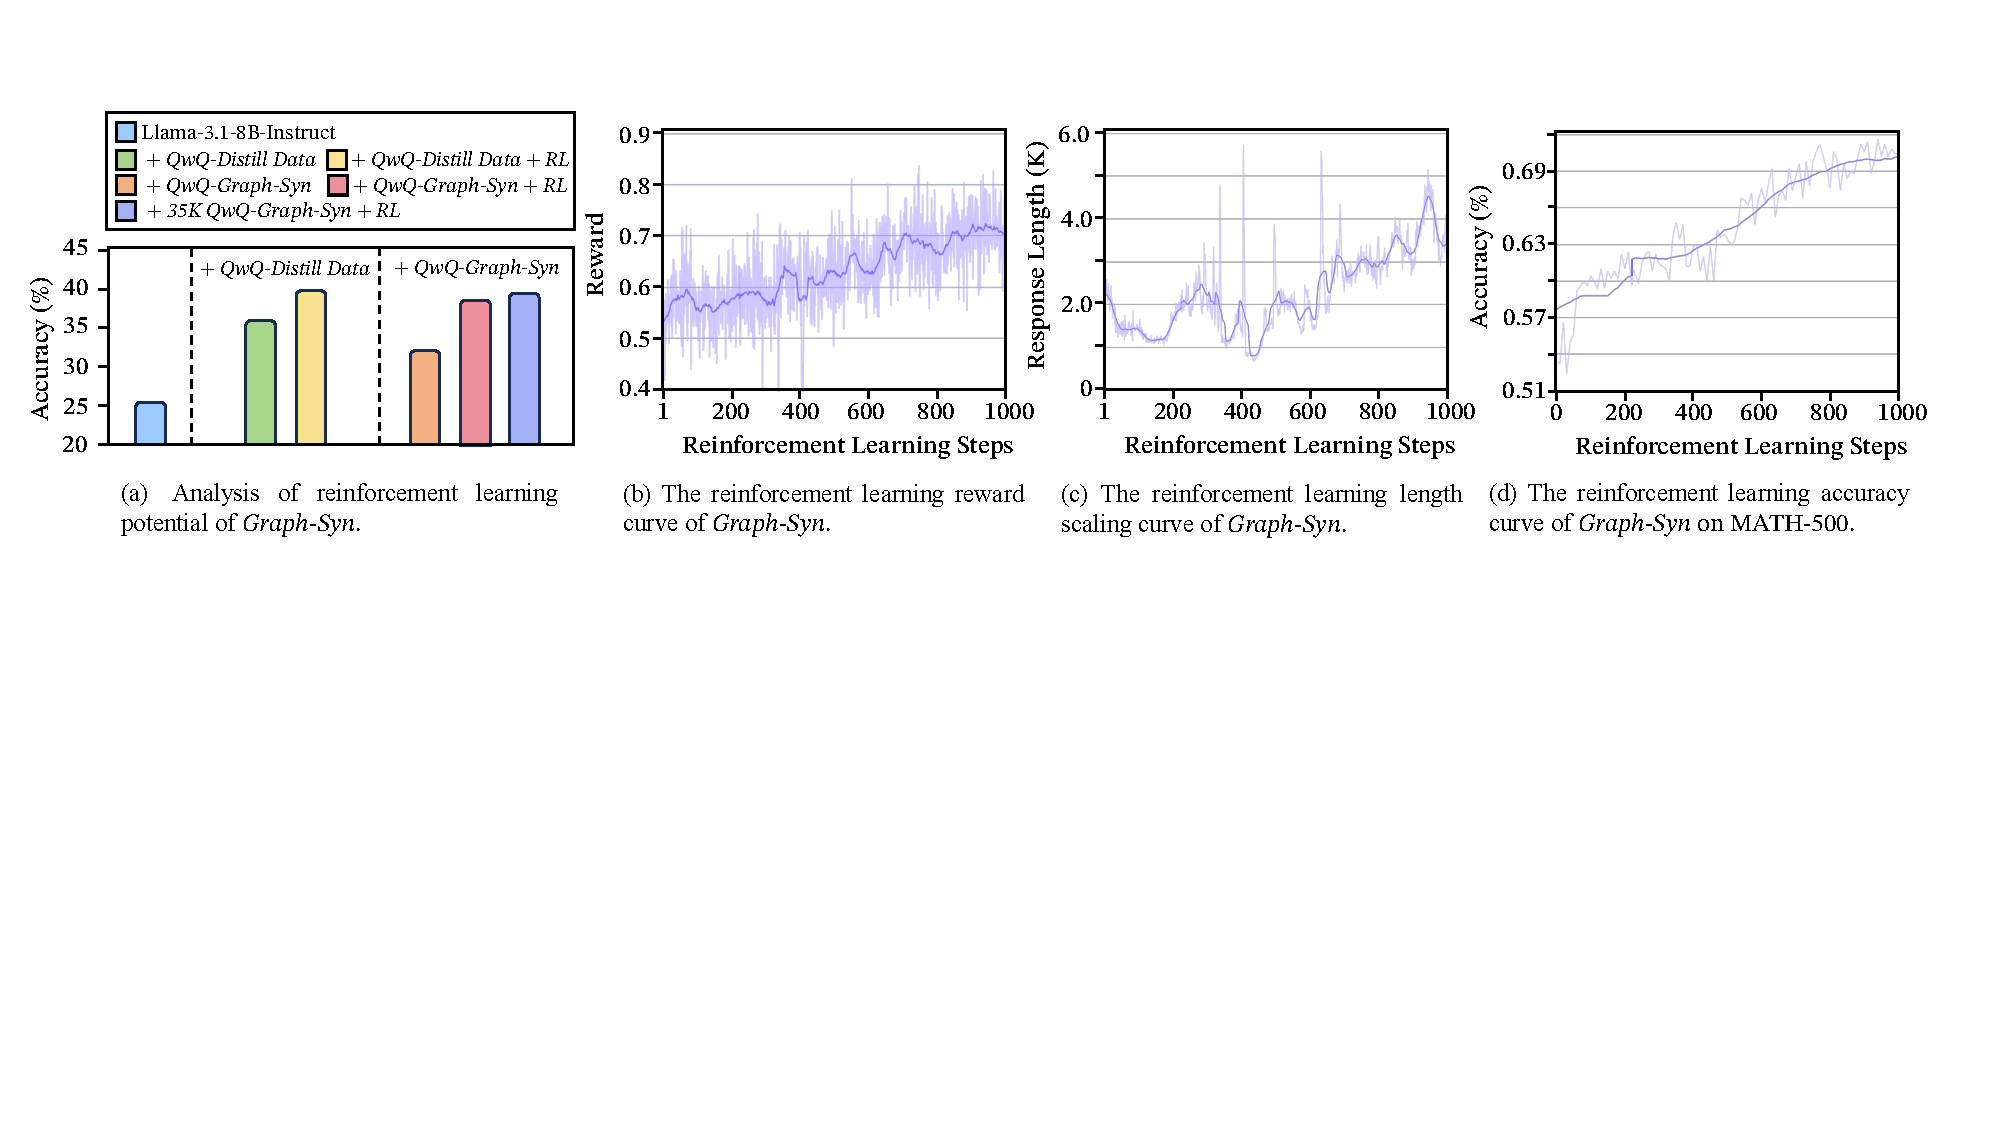
\includegraphics[width=0.98\textwidth]{figures/rl.pdf}
    
    \caption{以 \method 初始化的模型在强化学习阶段持续提升。更详细的 RL 结果见附录表~\ref{tab:rl_results}。}
    
    \label{fig:rl}
\end{figure*}

\section{合成化学：从零合成 Long CoT 分子}
LLM 可能在接触到显式、具结构的 Long CoT 轨迹后获得高级推理能力。但我们仍然不清楚：是否可以通过提示一个指令模型来稳定地诱导这种结构，而不依赖蒸馏。\vspace{-8pt}


\paragraph{\textbf{\method 方法论。}}
为此，我们提出 \method：把目标推理轨迹视作大分子结构，仅需指令 LLM 即可实现。该方法在图~\ref{fig:transfer} 所示的转移概率图上执行随机游走。该图由加强 Long CoT 的强推理模型提供四类推理行为的转移概率。\vspace{-8pt}


\paragraph{\textbf{\method 能合成有效的键结构。}}
为了验证是否可以仅依赖指令模型就学得 Long CoT 能力，我们在表~\ref{tab:synthesis_results} 中报告了基于 \method 生成数据训练的结果，其性能可以接近 QwQ 蒸馏。这表明，基于指令模型的合成同样能诱导有用的结构规律，从而以更低成本实现行为迁移。\vspace{-8pt}


\begin{figure*}[t]
    \centering
    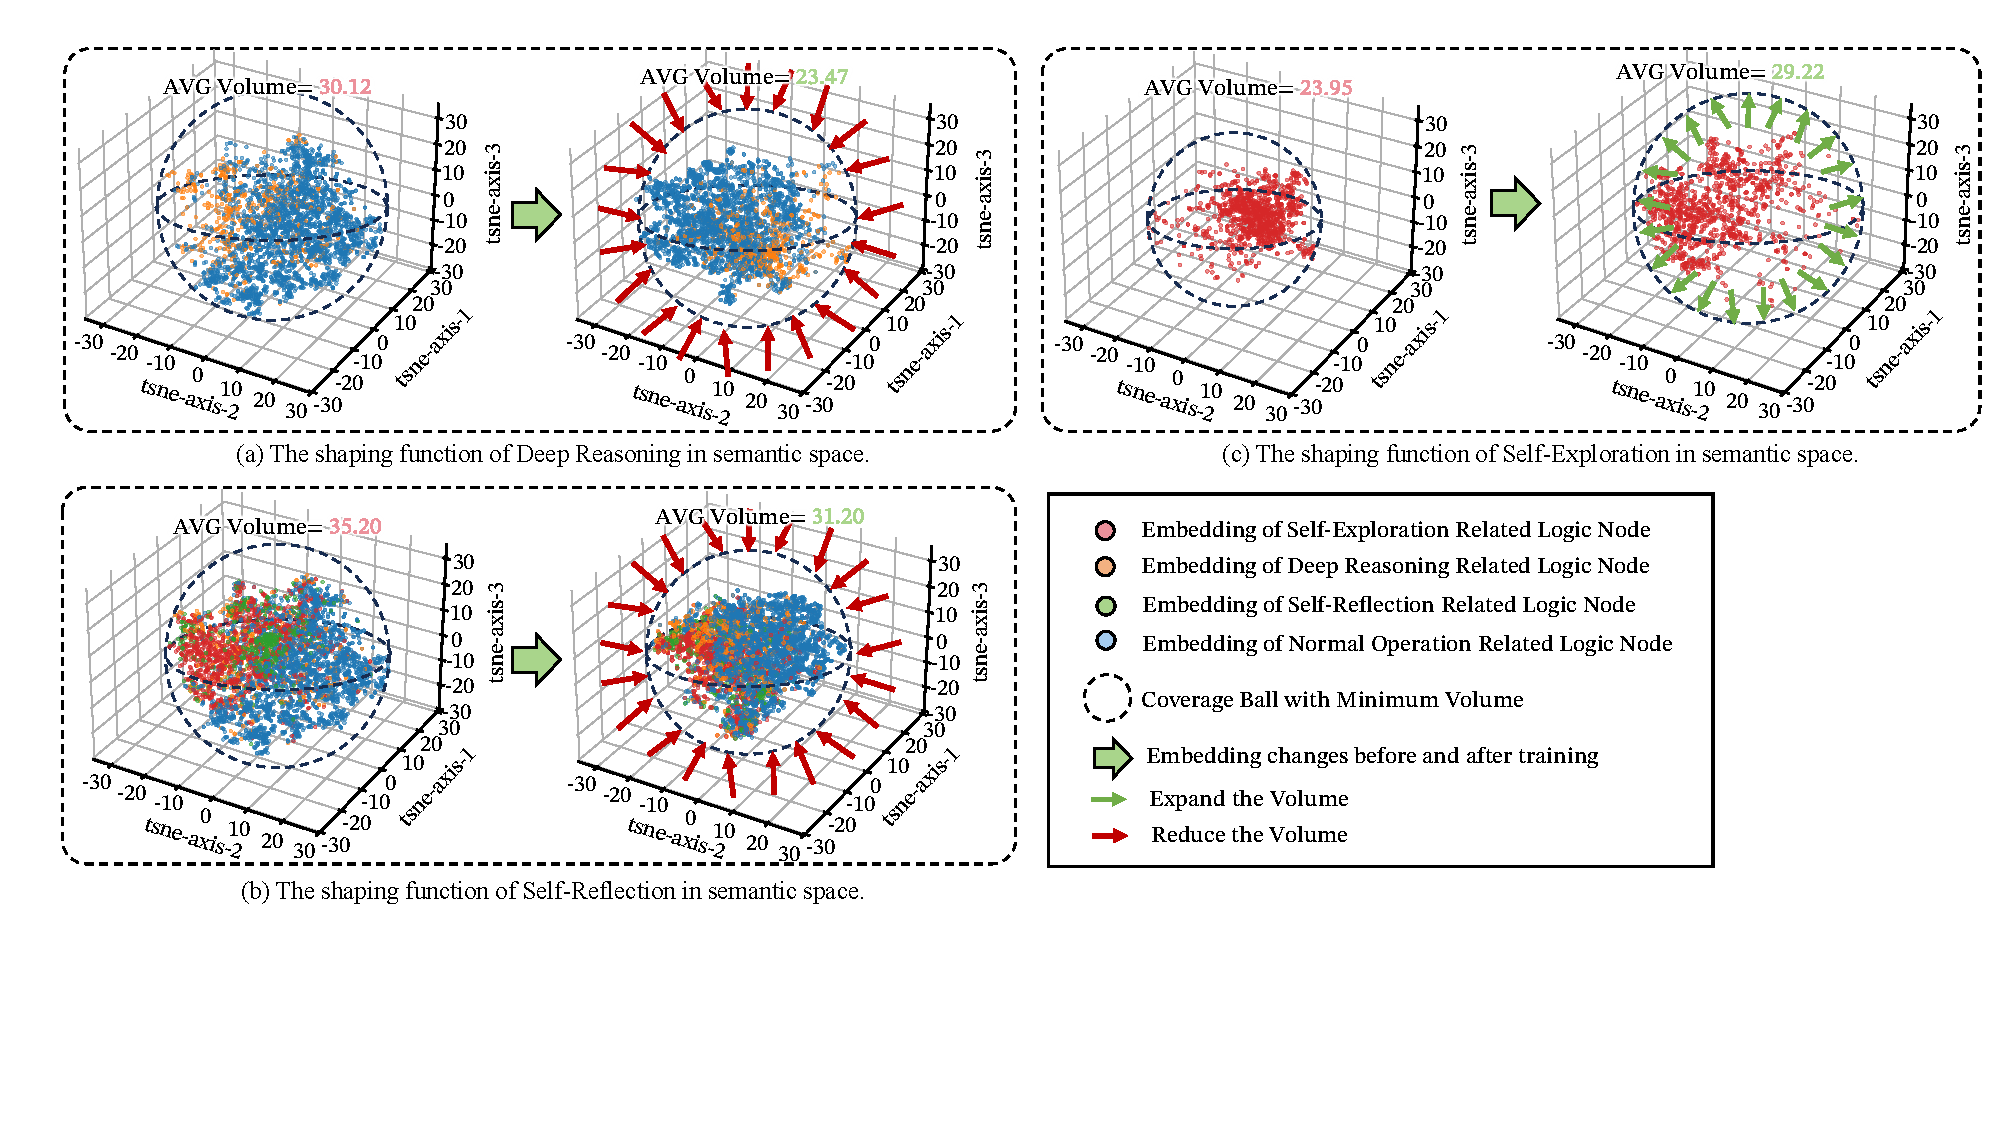
\includegraphics[width=0.98\textwidth]{figures/function.pdf}
    
    \caption{基于 Llama-3.1-8B-Instruct 及其 +QwQ-\method 版本在语义空间上的对比，展示不同键的作用。性能影响见附录图~\ref{fig:capability}。}
    
    \label{fig:function}
\end{figure*}

\paragraph{\textbf{\method 还能激发更强且持续提升的强化学习。}}
我们进一步评估 \method 初始化的 LLM 在强化学习（RL）中的潜力。相较于基座模型，\method 初始化的模型表现更佳。图~\ref{fig:rl}(a) 显示，它们在微调初期就能更平稳地提升，表明具备更强的即时推理与更可靠的 RL 适应能力。
此外，图~\ref{fig:rl}(b-d) 说明这些收益在长期 RL 训练中仍能持续，证明合成的 Long CoT 结构具有持久价值。这也进一步表明，该方法在多种认知任务中具有实用性。

\begin{TakeawayBox}{结论 4}
\begin{itemize}[leftmargin=16pt, itemsep=0pt, topsep=0pt]
    \item \method 无需 Long CoT 蒸馏数据即可合成匹配强教师转移分布的结构；
    \item 基于转移的 Long CoT 数据能够稳定收敛并接近蒸馏性能，证明纯指令级的合成就能以更低成本产生有效推理结构；
    \item 由合成结构初始化的模型在强化学习中表现更强、更持续，是在动态环境中进行持续学习的稳健起点。
\end{itemize} 
\end{TakeawayBox}
